\section{Introduction}
\label{sec:introduction}

As pre-trained models mature, an increasing share of advances in capabilities
such as agentic tool use and coding has come from post-training
\citep{openai_gpt55_2026,anthropic_opus48_2026,
kimi_k2_2025,glm5_2026}. The effectiveness of post-training, however, is
closely coupled to the environment in which a model is trained, evaluated, and
deployed
\citep{yao_second_half_2025,meta_harness_2026,
continual_harness_2026}. The data a model learns from, the tools it can use,
the users it serves, and the interactions it must support jointly shape the
behavior required of a deployed agent
\citep{when_cl_requires_learning_2026,continual_harness_2026,
meta_harness_2026}. These conditions vary across deployments and continue to
evolve over time, as new knowledge becomes available, new domains emerge, and
interaction state accumulates across episodes
\citep{tic_lm_2025,when_cl_requires_learning_2026,exg_2026}.

A common practice is centralized post-training, in which a model is optimized
over a bounded set of tasks and environments, aligned with the current harness,
and consolidated into a checkpoint for release. Training on a broad task
mixture can improve aggregate performance across tasks, but heterogeneous
objectives can also create cross-task interference when they compete through
shared parameters
\citep{badit_2026}. More fundamentally, the resulting system remains tied to
the task and environment distribution available during training, while new
knowledge, tools, user needs, and interactions continue to arrive after release
\citep{tic_lm_2025,when_cl_requires_learning_2026,
continual_harness_2026,exg_2026}. We see this as approximating a static optimum
rather than constituting genuine intelligence. What we consider genuine
intelligence is \emph{experiential intelligence}: the ability to learn from
experience accumulated in a real environment and to keep learning after
deployment
\citep{silver_sutton_experience_2025,yao_second_half_2025}.

Mind Lab is built for experiential intelligence. We use \emph{Personal
Intelligence} for the user-facing competence required when an agent works over
time for a particular person: using tools reliably, remembering constraints
across sessions, deciding when to ask a clarifying question and when to act,
and staying honest with the person on the other end of the conversation. These
behaviors describe the product target; experiential intelligence adds a
temporal requirement that deployment experience feeds a later model--harness
revision. Current agent-model training largely treats the target behaviors as
capabilities to develop before release and then hold fixed: the model is tuned
against a snapshot of the environment and shipped. Once deployed, the
resulting system has limited mechanisms for turning execution experience into
systematic improvement over time~\citep{exg_2026,continual_harness_2026}.
\macaron{} is our attempt to build that revision loop.

\paragraph{Adaptation and collaboration.}
Experiential intelligence, as we operationalize it, has two complementary
dimensions, and \macaron{} is built around both.

\emph{Adaptation} is pursued through recursive improvement over explicitly
versioned model--harness pairs: each version names a fixed model snapshot and
runtime configuration.
Recent approaches differ in where and how they make experience persistent.
Parametric continual-learning methods update model weights across changing
tasks or distributions
\citep{continual_learning_llm_survey_2026,tic_lm_2025,
when_cl_requires_learning_2026}. Memory- and state-based methods carry
trajectories, retrieved experience, or compact online states forward without
immediately modifying model parameters
\citep{jitrl_2026,delta_mem_2026,livemem_2026,
metis_2026,exg_2026}. Context- and harness-based methods instead update the
instructions, tools, skills, memory procedures, orchestration, or execution
structure surrounding the model
\citep{ace_2026,meta_harness_2026,continual_harness_2026,
recursive_harness_2026}.

\macaron{} connects harness adaptation with modular parametric adaptation: it
builds harder tasks from seeds, audits trajectories in the production harness,
searches the context configurations that shape behavior, and selects
trajectories for subsequent updates to specialist LoRA adapters. Adaptation is
therefore a property we seek across successive model--harness revisions rather
than in any single checkpoint. We use \emph{recursive improvement} in a bounded
and auditable sense: experience generated by one versioned model--harness
configuration is evaluated under an external contract and used to construct a
successor revision
\citep{rsi_survey_2026}. Repeating this process across successive revisions,
while measuring retention, transfer, and cumulative improvement, is the
longer-term continual-learning objective
\citep{continual_learning_llm_survey_2026,
when_cl_requires_learning_2026}.

\emph{Collaboration} is pursued through composition. Joint post-training over
heterogeneous tasks within a shared parameter space can create cross-task
interference, motivating a representation in which specialists remain
separable
\citep{badit_2026}. Existing approaches compose specialists at different
granularities: mixture-of-adapter systems select or combine LoRA specialists at
the task, sequence, or token level
\citep{lorauter_2026,molora_2026}, while multi-agent systems coordinate
complete model instances through routing, communication, discussion, or
response aggregation
\citep{multiagent_collaboration_survey_2025,rethinking_moa_2025}.
Mixture-of-LoRA (\molshort{}) occupies a different operating point: it keeps a
large base model frozen, layers specialist LoRA adapters on top
\citep{lora2022,lora_without_regret_2025}, and selects one specialist per user
turn through a shared runtime
\citep{mol_harness2026}.

\molshort{} demonstrates \emph{modular collaboration}. We reserve
\emph{collective intelligence} for the stronger setting in which independently
trained specialists contribute complementary capabilities, enabling the
composed system either to outperform its strongest constituent or to solve
tasks that no constituent can solve alone under a matched evaluation budget
\citep{rethinking_moa_2025,multiagentbench_2025,superminds_2026}.
Extending \molshort{} to include specialists trained by different teams or for
different users is the broader collective-intelligence objective.

Adaptation and collaboration are complementary dimensions of an evolving agent
system. Collaboration determines how distinct capabilities are represented,
selected, and composed, while adaptation determines how those capabilities and
the surrounding harness change in response to experience. Extending this
process across multiple generations, so that specialists, routing policies,
and harness configurations improve together while retaining prior capabilities,
remains a longer-term research direction
\citep{evolverouter_2026,evochamber_2026}.

\begin{figure}[t]
    \centering
    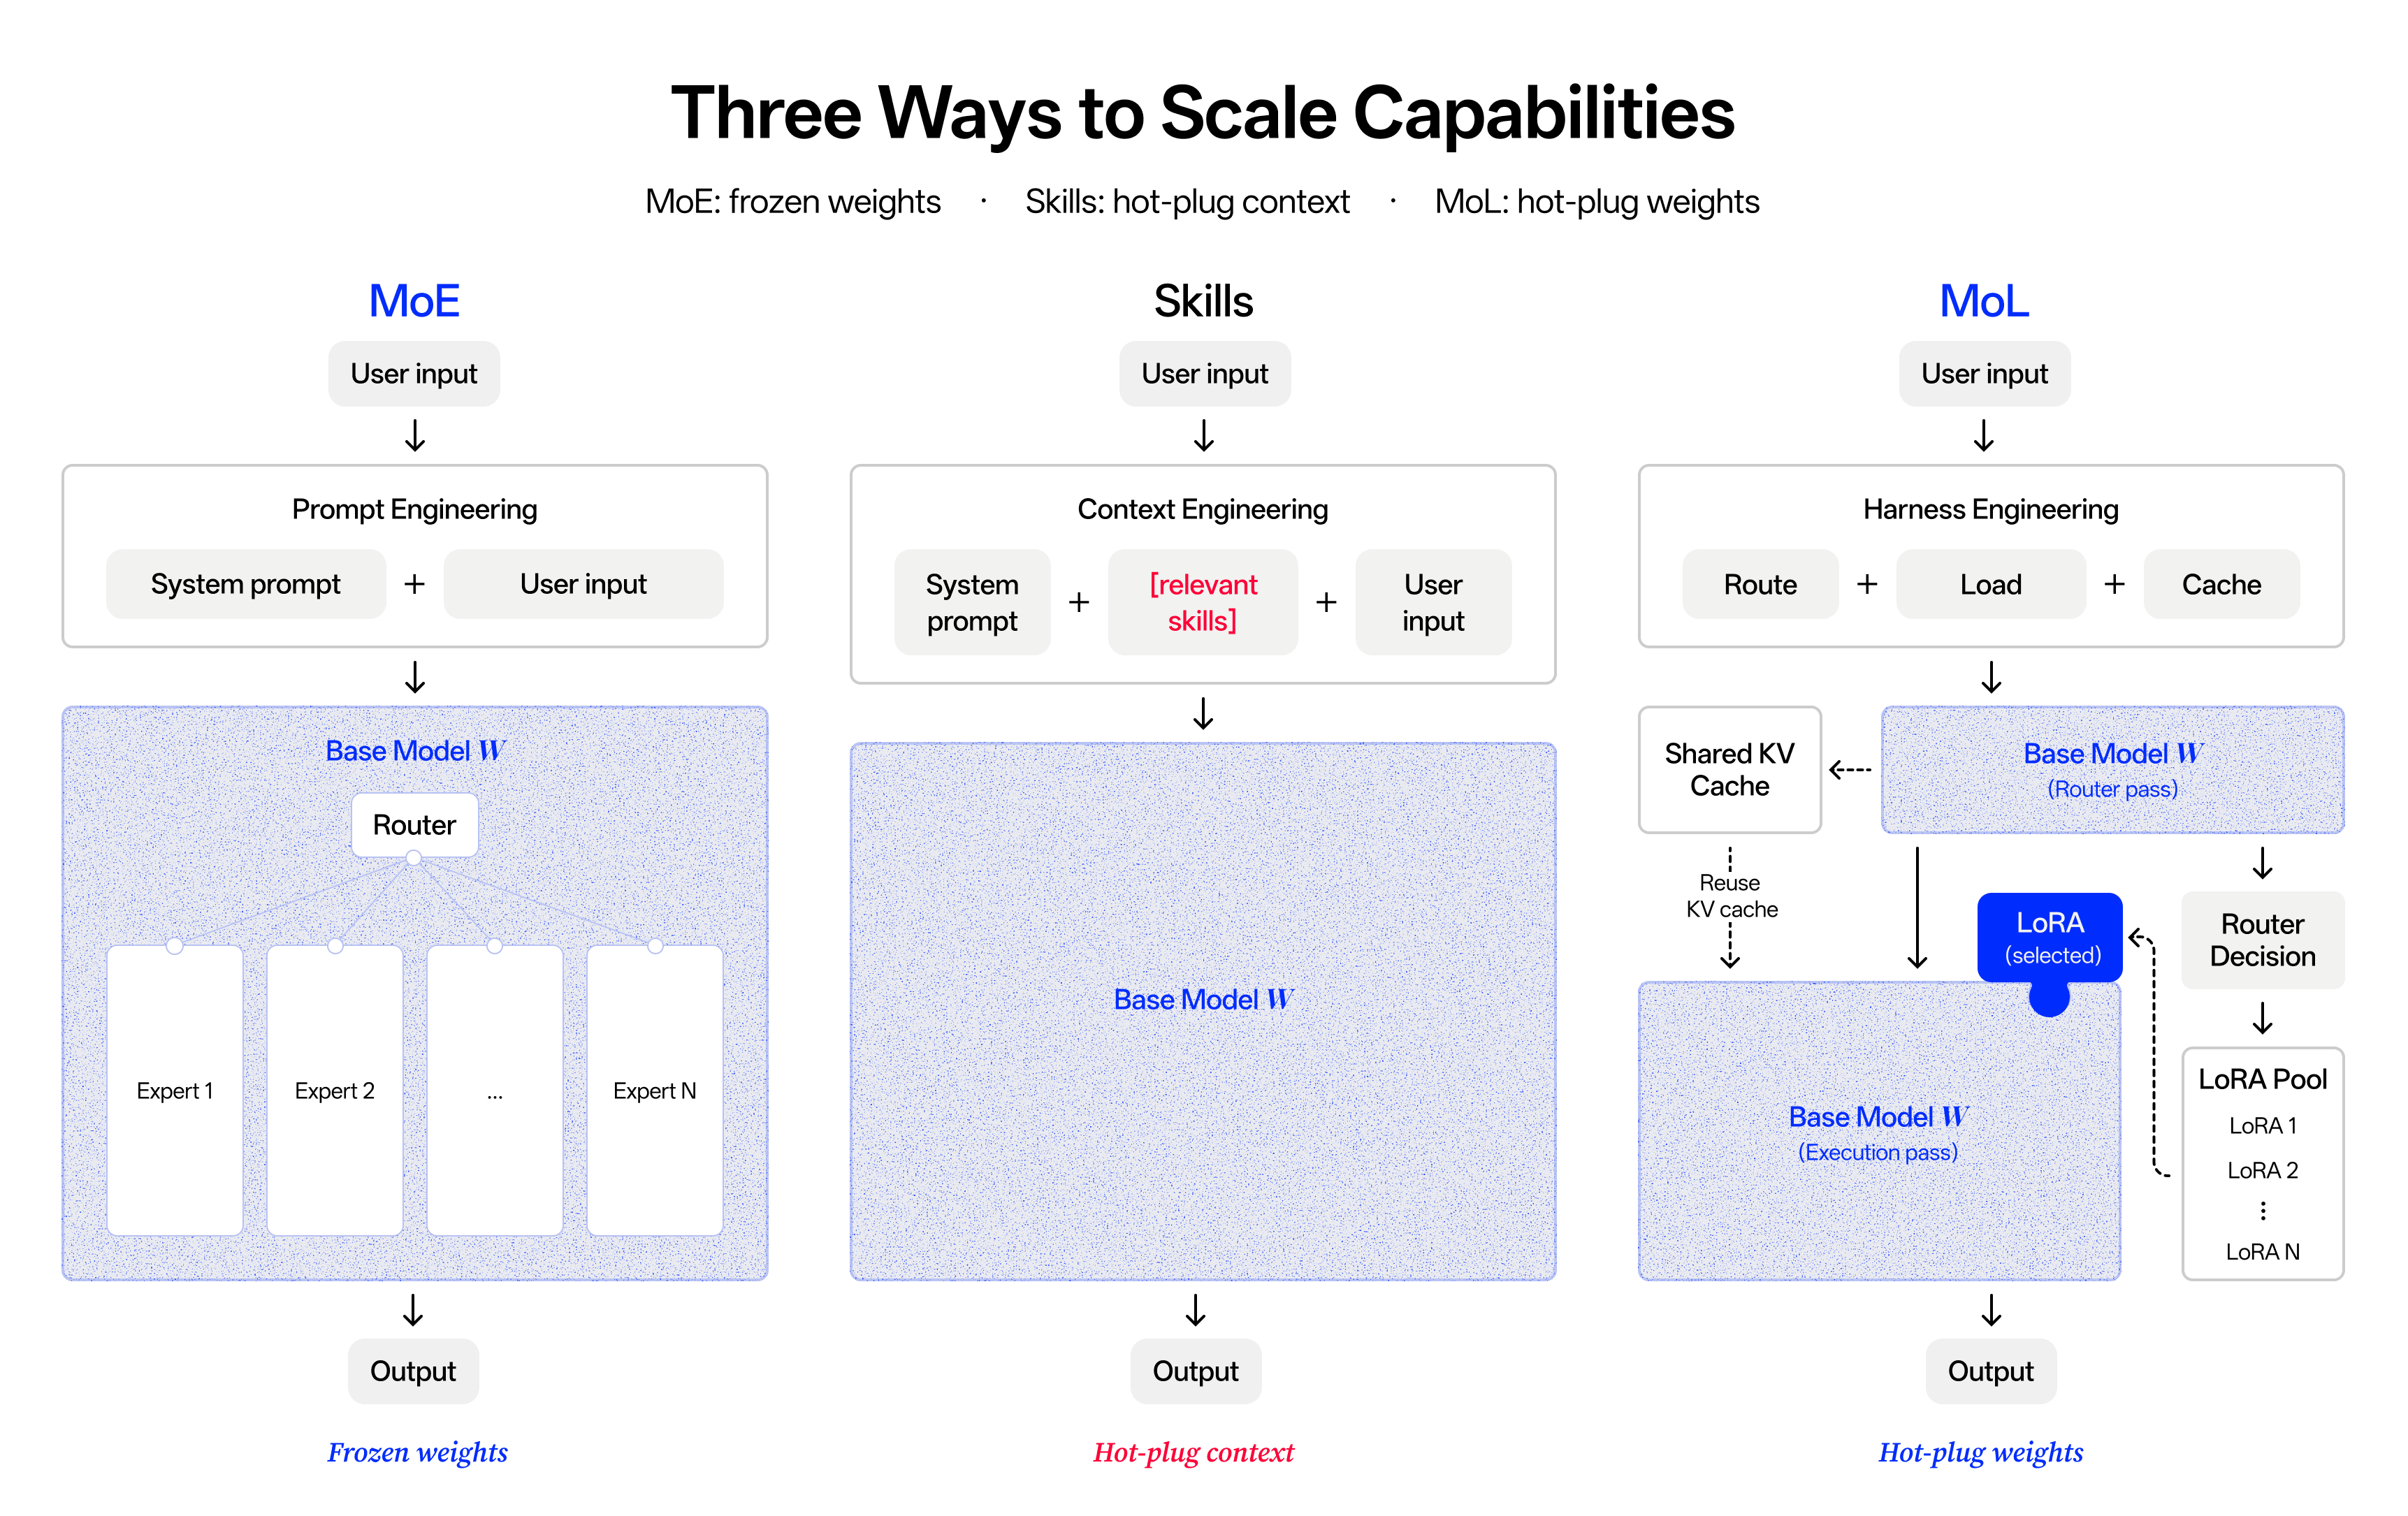
\includegraphics[width=0.95\linewidth]{figures/mol_three_ways.png}
    \caption{Three ways to scale model capability. Mixture-of-Experts (MoE) scales the base itself; skills scale scaffolding around a fixed model; \molshort{} (\mol) keeps the base frozen and composes specialist LoRA adapters through a Proxy-mediated routing loop. This separation is an implementation substrate for our continual-learning and collective-intelligence goals; the diagram is not a controlled comparison of the three alternatives.}
    \label{fig:mol_three_ways}
\end{figure}

\paragraph{Model family.}
\macaron{} is a family of open models rather than a single checkpoint.
\begin{itemize}[leftmargin=*]
  \item \venti{}: the flagship release, conventionally labeled 748B,
  consisting of a 744B GLM-5.2 base
  \citep{glm52_2026,glm5_2026} and four LoRA specialists. The label is
  release-facing; Section~\ref{sec:mol_specialists} gives the public
  stored-tensor count. It is
  post-trained with \mint{}
  \citep{lu2026announcing} and served through the \molshort{} harness
  \citep{mol_harness2026}.

  \item \tall{}: a 50B model post-trained from Qwen3.6
  \citep{qwen36_2026,qwen3_2025}, targeted at local deployment and
  lower-latency serving. It ships the same four-adapter \molshort{} design as
  \venti{}, with adapter placement and ranks chosen for Qwen3.6's MoE expert
  layout. Its public adapter configurations use a different rank and expert
  target set from \venti{}; the resulting aggregate is therefore reported as a
  rounded release footprint rather than inferred from base size alone.

  \item \codingventi{}: a coding-specialized build of \venti{} released
  by merging the coding LoRA directly into the base rather than serving it
  as a \molshort{} adapter.
\end{itemize}

The two \molshort{}-served variants share the same architectural pattern: a
frozen base, a small set of LoRA specialists, a Proxy-mediated route hop whose
label is emitted by L0, and a harness that stays close to production during both
training and serving. \codingventi{} is the single-specialist exception.

\paragraph{Contributions.}
This report describes \macaron{} as a co-designed system. Concretely, we
contribute:

\begin{itemize}[leftmargin=*]
  \item \textbf{\mol{} architecture.}
  A Proxy-mediated, per-turn composition scheme on top of a frozen base. The
  separation makes it possible to add LoRA specialists without retraining the
  base and to register specialists from different teams or users on one
  runtime. The shipped \venti{} model instantiates this architecture with four
  specialists; we report its routing functionality and serving cost, while
  continual improvement across generations and complementary gains from
  independently trained specialists remain evaluation targets described in
  Section~\ref{sec:disc_roadmap}. We release the serving harness at
  \texttt{MindLab-Research/Mixture-of-LoRA-Harness}
  \citep{mol_harness2026}.

  \item \textbf{Model--Harness Co-design and RSI.}
  We treat the harness as a first-class optimization target:
  \uifora{}
  \citep{ui4a2026} is a component-native harness for Generative UI,
  extending our prior schema-native work
  \citep{macaron_a2ui2026,a2ui_v08}; our REPL-based agent harness
  \citep{wu2026replharnesses} treats \emph{executable composition} and
  \emph{validated reuse} as the interface between the model and its tools; and
  the \hcp{} makes runtime selection, tools, skills, prompts, hooks, sessions,
  and workspace resources portable and auditable. \mindforge{}, our agentic RL
  framework, runs a three-stage loop of task discovery, trajectory expansion,
  and linked model/configuration updates against that harness. The experiment
  reported here isolates only the Expansion stage: the model remains frozen and
  no optimizer step is taken. In this fixed-model harness-search study, adaptive
  search reaches cumulative coverage of $122/122$ selected base-failure tasks,
  while the stronger of two full-set single-configuration sweeps reaches
  $11/122$ (Section~\ref{sec:rsi_coverage}). Because task targeting and error
  rates differ across phases, this result measures configuration-search coverage,
  not improvement produced by the full RSI training cycle.
  R3 rollout routing replay
  \citep{chiang2026routerreplay,r3_moe_router2025}, DSA integration fixes
  \citep{stevenchiang2026supportglm5inmint}, and IcePop-style token masking
  \citep{ling_every_step2025} address rollout--learner mismatch on the sparse
  base.

  \item \textbf{Infrastructure.}
  We provide the \mint{} post-training platform
  \citep{lu2026announcing}, including adapter-revision handoff, a measured
  million-entry addressable catalog, and trillion-parameter-class
  model-parallel paths, together with \longstraw{}
  \citep{zhou2026longstrawlongcontextrl2m}, an architecture-aware
  response-only execution stack with reported multi-million-token operating
  points under fixed GPU inventories. These measurements come from the
  companion systems reports rather than matched \macaron{} training runs.

  \item \textbf{Personal Intelligence benchmarks.}
  We introduce \chatbench{}, which evaluates context-conditioned agent
  conversation, and \livingbench{}, which evaluates stateful simulated
  personal-life assistance under evolving conditions. Both evaluate
  interaction trajectories rather than isolated answers.

  \item \textbf{Evaluation.}
  We evaluate \macaron{} across Personal Intelligence
  (\chatbench{}, \livingbench{}), agent, coding, and GenUI tracks
  against six comparison models. We distinguish scores reproduced in our
  harness from values taken from public reports, and treat the internal
  Personal Intelligence results as in-distribution evidence rather than as a
  general-capability comparison (Section~\ref{sec:results}).
\end{itemize}

\paragraph{Report structure.}
Section~\ref{sec:mol} describes collaboration through the \molshort{}
architecture, including its mechanisms for specialist composition and its
paths toward continual learning and collective intelligence.
Section~\ref{sec:algorithm} describes adaptation through Model--Harness
Co-design (\uifora{}, the REPL harness, and \hcp{}) and the recursive
self-improvement loop. Section~\ref{sec:infrastructure} covers the \mint{}
lifecycle, the \longstraw{} execution path, and sparse-base mismatch controls.
Section~\ref{sec:benchmarks} introduces the benchmarks we evaluate on,
Section~\ref{sec:results} reports the results, and
Section~\ref{sec:discussion} discusses limitations and the roadmap.
